\documentclass[slides,compress]{beamer}
\usepackage{graphicx,amsmath,hyperref}
\usepackage{verbatim}

\usepackage[normalem]{ulem}

\usetheme{default}
\useinnertheme{rectangles}

%\title{\huge Radiation Damage Analysis with $R_{\rm{cp}}(d)$}
\title{\huge A Novel Statistic for Radiation Damage Analysis}
\subtitle{\large ACA 2012}

\author{Graeme Winter}
\institute{Diamond Light Source}
\date{July 2012}

\begin{document}

\setbeamertemplate{background}{

\includegraphics[width=\paperwidth,height=\paperheight]
{diamond-background.png}
}

\frame{\maketitle}

\frame{
\frametitle{Overview}
\begin{itemize}
\item{Strategy, background, caveats}
\item{Review of statistics}
\item{Example cases}
\item{New statistic - $R_{cp}(d)$}
\item{More example cases}
\item{Discussion, acknowledgements}
\end{itemize}
}

\frame{
\frametitle{Caveats}
\begin{itemize}
\item{All data described processed with xia2 / XDS i.e. using
    ``standard methods''}
\item{All this will show is a new tool and some instances where it
    could be useful} 
\item{All calculations independent of data analysis program used}
\item{Program to perform these calculations included with xia2:
    pychef}
\end{itemize}
}

\frame{
\frametitle{Strategy}
\begin{itemize}
\item{Radiation damage gives rise to lots of changes}
\item{Will only discuss changes to measured \emph{intensities}
    i.e. not
\begin{itemize}
\item{Changes to unit cell}
\item{Relative $B$-factor in scaling}
\item{Vanishing diffraction}
\end{itemize}
}
\item{Assume sufficient data for scaling, analyse after corrections
    applied, no assumptions about scaling \emph{program}}
\item{Looking to answer the question: would this data set have been
    more useful if I stopped collecting data earlier - balancing:
\begin{itemize}
\item{Gains from additional measurements i.e. multiplicity}
\item{Losses due to systematic changes reducing signal}
\end{itemize}
}
\item{Assume sufficient multiplicity that above question is meaningful
  (same as zero-dose)}
\end{itemize}
}

\frame{
\frametitle{$R_{\rm{merge}}$}
\begin{equation}
R_{\rm{merge}}(i) = 
\frac{\sum_{\underline{h}} \sum_{j: i = \rm{image}} | I_{{\underline{h}}j} - 
\overline{I}_{\underline{h}} |}
{\sum_{\underline{h}} \sum_{j: i = \rm{image}} I_{{\underline{h}}j}}
\end{equation}
Measures: how well reflections on frame $i$ agree with the average
values of those reflections. This is reported by Scala.
}

\frame{
\frametitle{$R_{\rm{d}}$, Diederichs (2006)}
\begin{equation}
R_d = \frac{\sum_{{\underline{h}}} \sum_{|b_j - b_i| = d}
|I_{\underline{h}j} - I_{\underline{h}i}|}
{\sum_{{\underline{h}}} \sum_{|b_j - b_i| = d}
\frac{1}{2}|I_{\underline{h}j} + I_{\underline{h}i}|}
\end{equation}
Measures: how well reflections separated by $d$ frames agree. This is
reported by XDSSTAT.
}

\frame{
\frametitle{Application to Example Sets}
\begin{itemize}
\item{Straightforward thaumatin example}
\item{Radiation-damaged SAD}
\item{Radiation-damaged MAD}
\end{itemize}
}

\frame{
\frametitle{Example 1: thaumatin}
\begin{itemize}
\item{A dull, native, good-quality sample}
\item{Recorded during beamline setup at Diamond I03}
\item{900 frames $\times 0.1^{\circ}$}
\item{Purpose: illustrate properties of existing residuals}
\end{itemize}
}

\frame{
\frametitle{Thaumatin: $R_{\rm{merge}}$}
\begin{center}
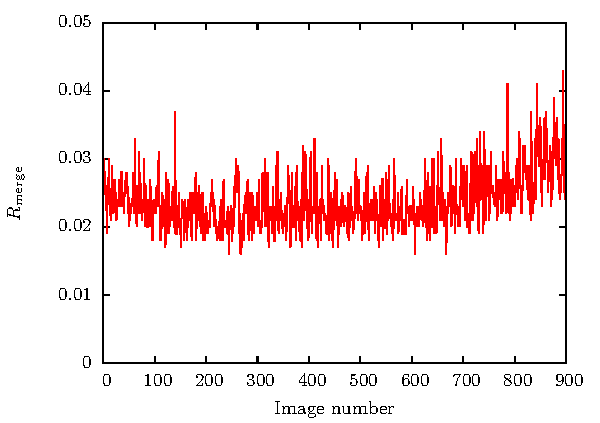
\includegraphics[scale=1.0]{figures/simple2/rmerge.pdf}
\end{center}
}

\frame{
\frametitle{Thaumatin: $R_d$}
\begin{center}
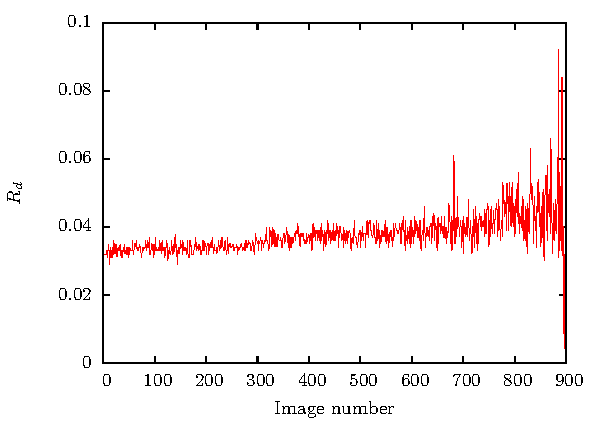
\includegraphics[scale=1.0]{figures/simple2/rd.pdf}
\end{center}
}

\frame{
\frametitle{Example 2: radiation damaged SAD data}
\begin{itemize}
\item{High multiplicity SAD data set recorded from \emph{Helix pomatia
      Agglutinin} at ESRF beamline ID14EH2 by Ed Mitchell as part of
    ongoing research}
\item{$1440^{\circ}$ of data, of which $720^{\circ}$ were used in the
    structure solution due to radiation damage}
\item{Symmetry is $H32$, so the data have $\sim 80$-fold multiplicity}
\end{itemize}
}

\frame{
\frametitle{HPA: $R_{\rm{merge}}$}
\begin{center}
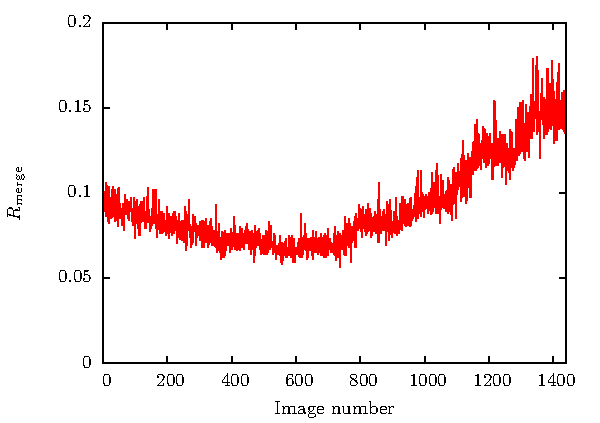
\includegraphics[scale=1.0]{figures/hpa/rmerge.pdf}
\end{center}
}

\frame{
\frametitle{HPA: $R_d$}
\begin{center}
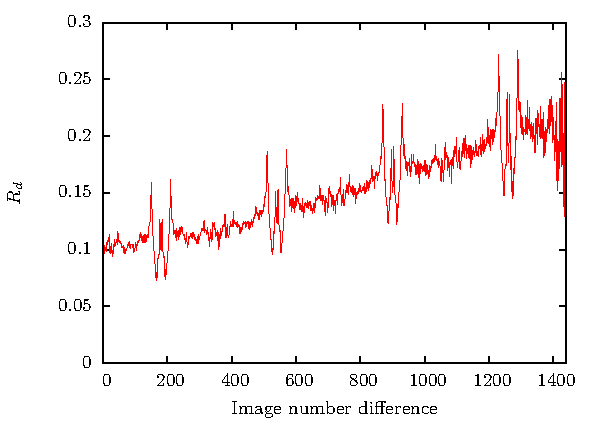
\includegraphics[scale=1.0]{figures/hpa/rd.pdf}
\end{center}
}

\frame{
\frametitle{Example 3: radiation damaged MAD data}
\begin{itemize}
\item{JCSG target TB0541B}
\item{8 Se / 200 AA, 3 $\lambda$ MAD with inverse beam on inflection
    and low energy remote}
\item{Classic example of nasty radiation damage}
\end{itemize}
}

\frame{
\frametitle{2ISB: $R_{\rm{merge}}$}
\begin{center}
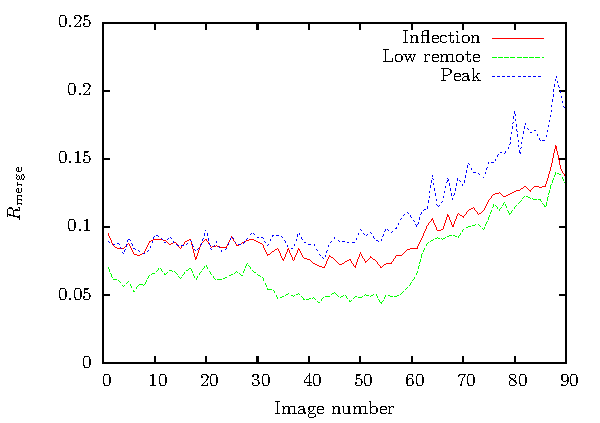
\includegraphics[scale=1.0]{figures/2isb/rmerge.pdf}
\end{center}
}

\frame{
\frametitle{2ISB: $R_d$}
\begin{center}
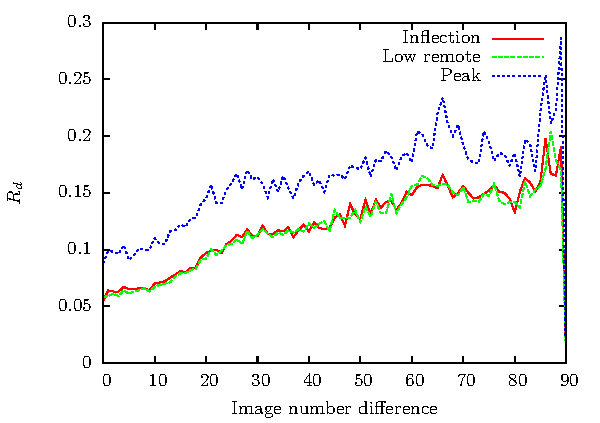
\includegraphics[scale=1.0]{figures/2isb/rd.pdf}
\end{center}
}

\frame{
\frametitle{Review}
\begin{itemize}
\item{Stats behave as expected - presence or absence of radiation
    damage is clear}
\item{No information provided so far about subset options i.e. when I
    clearly do have radiation damage, what to do?}
\item{MAD data sets not considered very gracefully}
\end{itemize}
}

\frame{
\frametitle{Novel Statistic}
\begin{itemize}
\item{Question: could things have been better if I had stopped
    collecting data earlier? I.e. think about wall-clock \emph{time}}
\item{$R_{\rm{merge}}$ contains time information, $R_d$ shows
    difference information, wouldn't it be great to have both?}
\item{Including how \emph{complete} the data are would also be
    important}
\end{itemize}
}

\frame{
\frametitle{Properties}
\begin{itemize}
\item{Computing pairwise differences avoids need for average value}
\item{Integrating differences up to some dose $d$ reproduces
    experiment}
\item{Organising in terms of dose, integrating across wavelengths and
    sweeps allows evolution of sample to be described}
\item{While performing analysis, compute completeness (anomalous and
    native) for each wavelength as function of $d$}
\end{itemize}
}

\frame{
\frametitle{$R_{cp}(d)$, \emph{Cumulative-Pairwise} Residual}
\begin{equation}
R_{cp}(d) = \frac{\sum_{\lambda} \sum_{\underline{h}} \sum_{
{i \neq j}, i:d_i \leq d, j:d_j \leq d} |I_{\underline{h}i} - 
I_{\underline{h}j}|}
{\sum_{\lambda} \sum_{\underline{h}} 
\sum_{i \neq j, i:d_i \leq d, j:d_j \leq d} \frac{1}{2}|I_{\underline{h}i} + 
I_{\underline{h}j}|}
\end{equation}
Measures: including data to a point $d$, how internally consistent are
the measurements?
}

\frame{
\frametitle{In English?}
\begin{itemize}
\item{For each wavelength, for each $HKL$, accumulate generally
    how different the intensities are up to some dose $d$}
\item{Then plot this as a function of $d$}
\item{And while you're there record how complete wavelengths are up to
    point $d$ too...}
\end{itemize}
}

\frame{
\frametitle{Application to Thaumatin}
\begin{center}
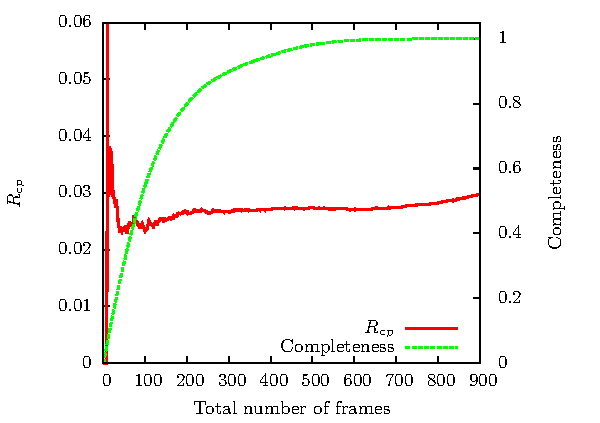
\includegraphics[scale=1.0]{figures/simple2/rcp2.pdf}
\end{center}
}

\frame{
\frametitle{Comments and observations}
\begin{itemize}
\item{At the start always 'noisy' as there are few pairs - only trust
    once data are e.g. 50\% complete - this is very similar noise to
    the end of an $R_d$ plot}
\item{Most interesting is what happens after the data are fairly
    complete - in this case, nothing}
\item{Even more interesting is to use \emph{dose} as the baseline
    rather than batch, though equivalent for SAD}
\end{itemize}
}

\frame{
\frametitle{Application to MAD data}
\begin{center}
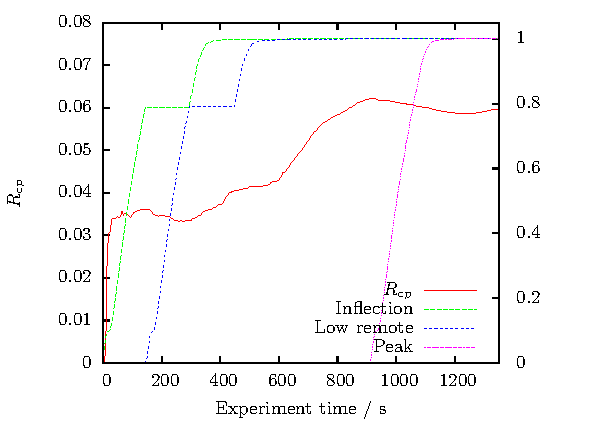
\includegraphics[scale=1.0]{figures/2isb/rcp2.pdf}
\end{center}
}

\frame{
\frametitle{Interpretation}
\begin{itemize}
\item{Full three wavelength data has high residual (i.e. after 1350s)}
\item{After 600s we have two complete wavelengths, much lower residual}
\end{itemize}
}

% FIXME merging stats for 2-wave and 3-wave processing - N.B. both
% phase fine with shelx c/d/e though

\frame{
\frametitle{Application to HPA}
\begin{center}
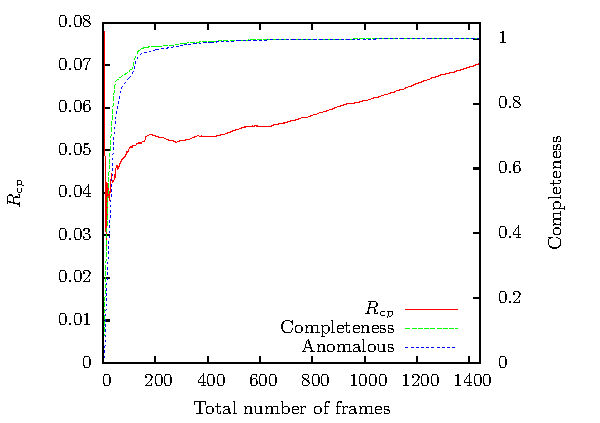
\includegraphics[scale=1.0]{figures/hpa/rcp2.pdf}
\end{center}
}

\frame{
\frametitle{Interpretation}
\begin{itemize}
\item{Time equivalent to number of frames}
\item{Complete data (anomalous, native) pretty early on}
\item{$R_{\rm{cp}}$ appears to increase systematically $\sim 400$
    images - just over one full rotation}
\item{One Zn site on special position - anomalous difference Patterson
    easy to interpret}
\item{Processed data set 32 times - $0^{\circ} - 45^{\circ}$,
    $0^{\circ} - 90^{\circ}$, ..., $0^{\circ} - 1440^{\circ}$ to fixed
  resolution limit (1.65\AA), used 30\AA\ to 3\AA\ to compute
  Patterson}
\end{itemize}
}

\frame{
\frametitle{HPA Anomalous Difference Patterson}
\begin{center}
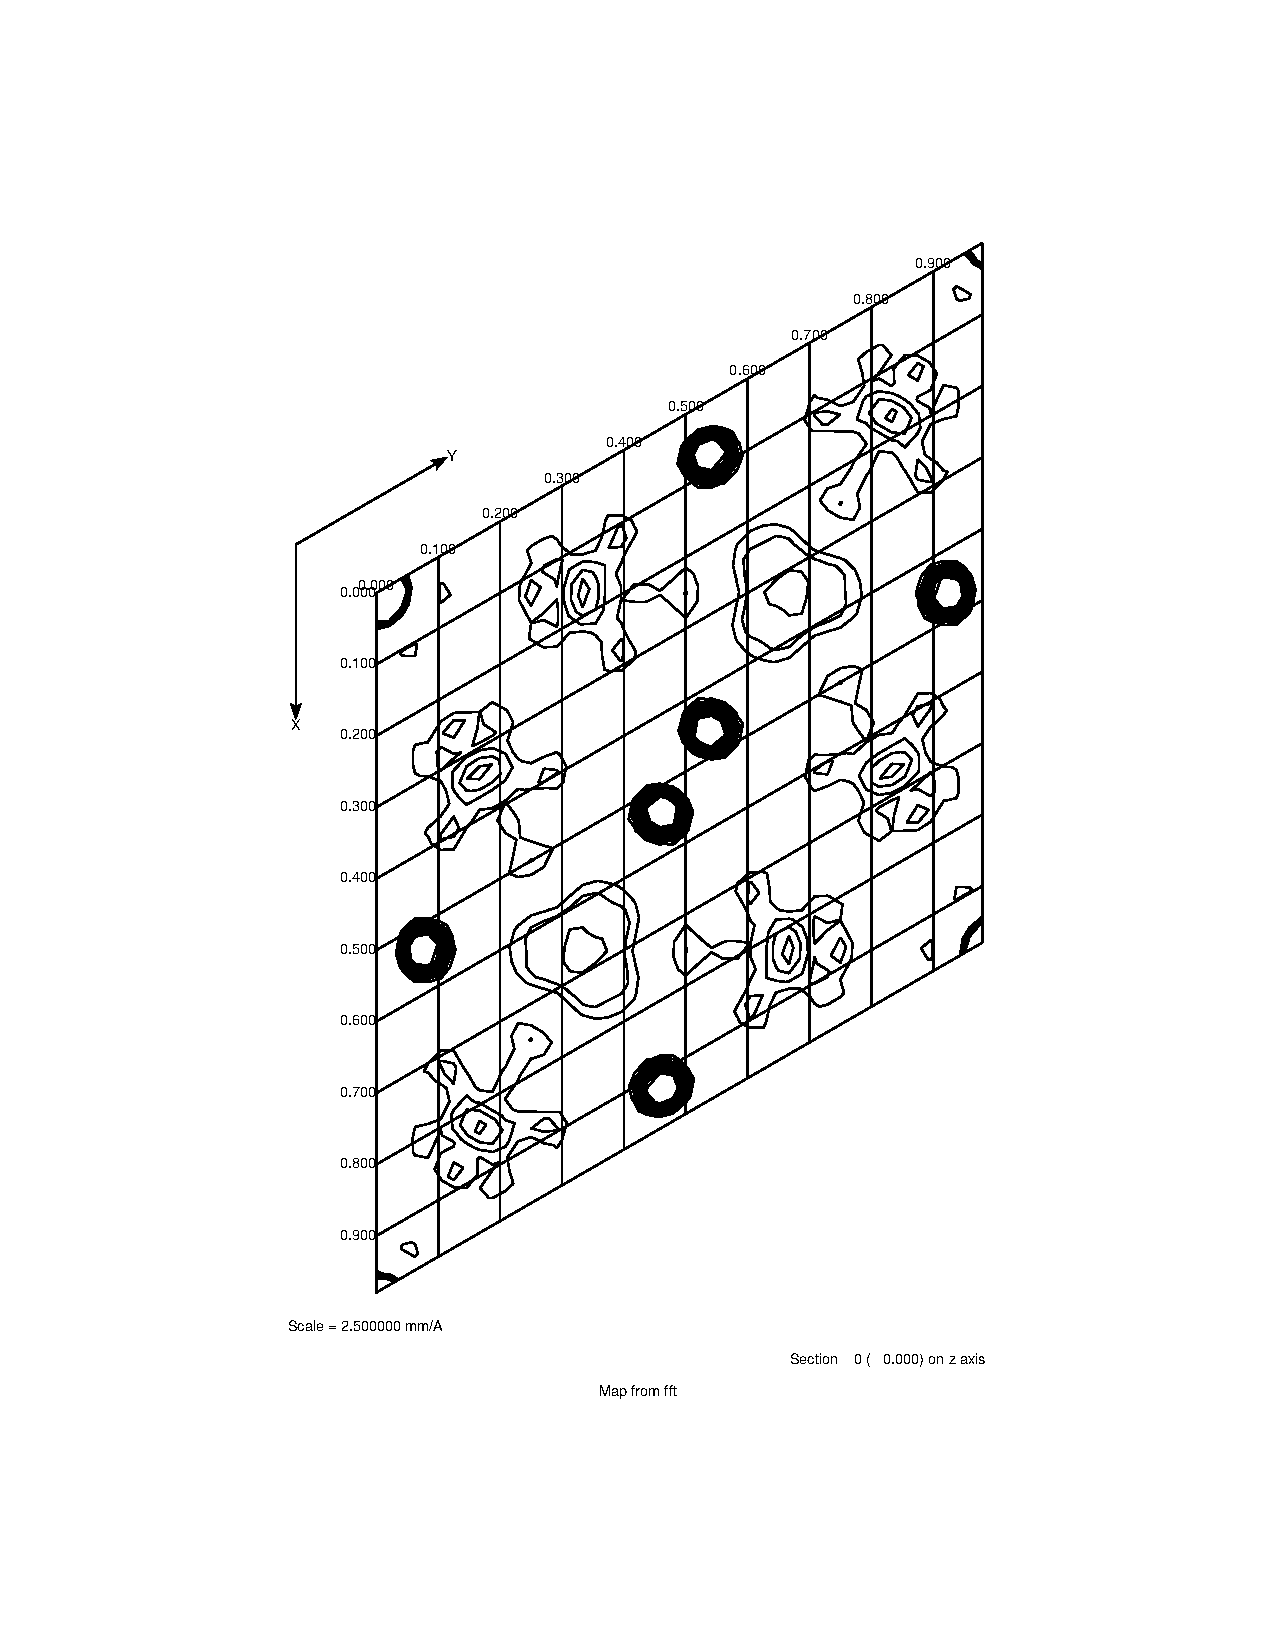
\includegraphics[scale=0.33]{figures/hpa/harker.pdf}
\end{center}
}

\frame{
\frametitle{Peak Height / $\sigma$}
\begin{center}
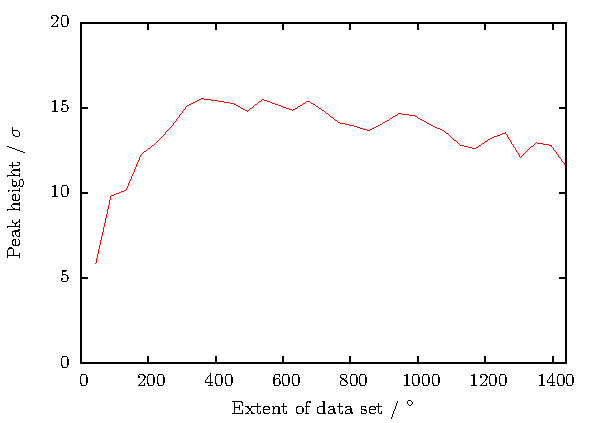
\includegraphics[scale=1.0]{figures/hpa/patterson_height.pdf}
\end{center}
}

\frame{
\frametitle{Interpretation}
\begin{itemize}
\item{After $\sim 360^{\circ}$ radiation damage becomes measurable}
\item{Complete subset around here gives ``most internally consistent''
  representation of the sample}
\item{Peak in anomalous difference Patterson using this much data}
\item{N.B. phasing works with subset, full data set, just using SHELX
    C/D/E}
\item{Zero-dose gave peak height of 16.07$\sigma$ - slightly better
    than the $360^{\circ}$ set but with $4\times$ the measurements used}
\end{itemize}
}

\frame{
\frametitle{Summary to date}
\begin{itemize}
\item{Looked at some examples}
\item{Showed new statistic}
\item{Illustrated statistic may be useful, perhaps more useful than
    $R_{\rm{merge}}$ \emph{vs.} batch and complementary to $R_d$}
\item{No cases shown where the insoluble becomes soluble - let's fix
    that}
\end{itemize}
}

\frame{
\frametitle{Unpublished Example - Au soak SAD}
\begin{itemize}
\item{Example from Christian Siebold at STRUBI}
\item{Measured at Diamond Light Source I03 using Pilatus 6M}
\item{Native data available, issue with this data set is substructure
    determination for phasing}
\end{itemize}
}

\frame{
\small
\begin{tabular}{lr@{.}lr@{.}lr@{.}l}
High resolution limit & 2 & 01 & 8 & 98 & 2 & 01 \\
Low resolution limit & 29 & 85 & 29 & 84 & 2 & 06 \\
Completeness & 71 & 2 & 97 & 3 & 13 & 5 \\
Multiplicity & 5 & 3 & 6 & 0 & 2 & 1 \\
I/sigma & 14 & 7 & 21 & 6 & 2 & 3 \\
Rmerge & 0 & 063 & 0 & 043 & 0 & 405 \\
Rmeas(I) & 0 & 086 & 0 & 067 & 0 & 707 \\
Rmeas(I+/-) & 0 & 076 & 0 & 052 & 0 & 568 \\
Rpim(I) & 0 & 034 & 0 & 027 & 0 & 470 \\
Rpim(I+/-) & 0 & 041 & 0 & 028 & 0 & 397 \\
Wilson B factor & 33 & 264 & & & & \\
Partial bias & 0 & 000 & 0 & 000 & 0 & 000 \\
Anomalous completeness & 65 & 1 & 97 & 6 & 10 & 6 \\
Anomalous multiplicity & 2 & 9 & 3 & 3 & 1 & 1 \\
Anomalous correlation & 0 & 388 & 0 & 613 & 0 & 690 \\
Anomalous slope & 1 & 589 & 0 & 000 & 0 & 000 \\
Total observations & 40714 &  & 775 &  & 228 &  \\
Total unique & 7685 &  & 130 &  & 111 &  \\
\end{tabular}
}

\frame{
\frametitle{Au soak: $R_{\rm{merge}}$}
\begin{center}
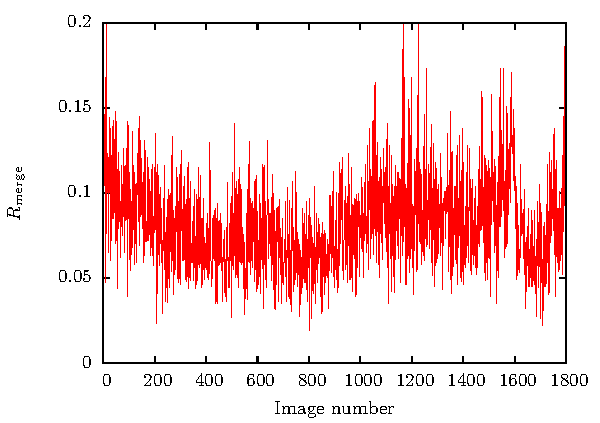
\includegraphics[scale=1.0]{figures/gold/1800_rmerge.pdf}
\end{center}
}

\frame{
\frametitle{Au soak: $R_d$}
\begin{center}
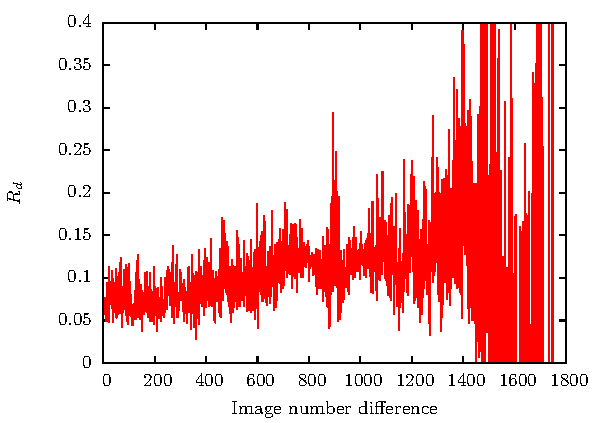
\includegraphics[scale=1.0]{figures/gold/1800_rd.pdf}
\end{center}
}

\frame{
\frametitle{Per-image analysis (DISTL)}
\begin{center}
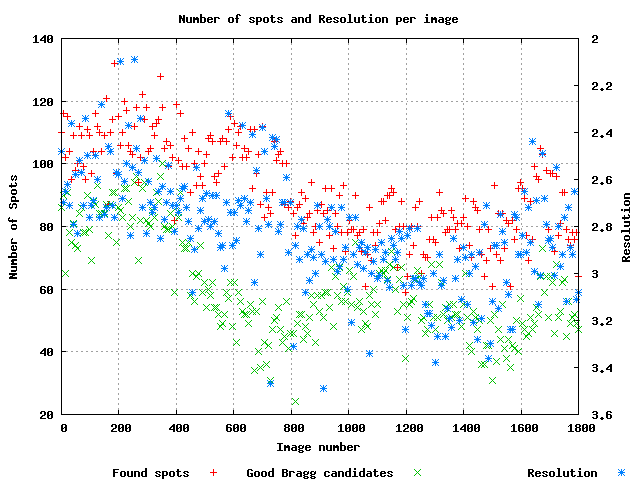
\includegraphics[scale=0.45]{figures/gold/pia.png}
\end{center}
}

\frame{
\frametitle{Interpretation}
\begin{itemize}
\item{Detector too far back - low completeness at high resolution}
\item{Merging stats reasonable, clearly we have some radiation damage}
\item{What does $R_{\rm{cp}}$ say?}
\end{itemize}
}

\frame{
\frametitle{Au soak: $R_{\rm{cp}}$}
\begin{center}
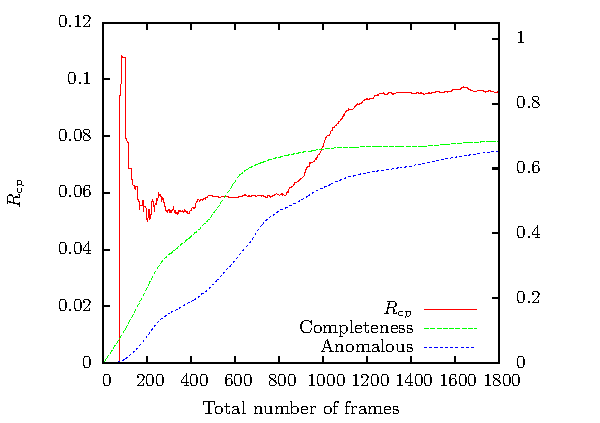
\includegraphics[scale=1.0]{figures/gold/1800_rcp2.pdf}
\end{center}
}

\frame{
\frametitle{Clear radiation damge}
\begin{itemize}
\item{Clear radiation damage according to this measure}
\item{Data essentially as complete as they can be half way through}
\item{Assert: using 900 frames / $180^{\circ}$ of the data will
    work better than the full set}
\item{Test: use SHELXD (via ``Fast EP'' at Diamond)}
\end{itemize}
}

\frame{
\small
\begin{tabular}{lr@{.}lr@{.}lr@{.}l}
High resolution limit & 2 & 01 & 8 & 98 & 2 & 01 \\
Low resolution limit & 29 & 83 & 29 & 83 & 2 & 06 \\
Completeness & 70 & 9 & 95 & 1 & 12 & 5 \\
Multiplicity & 2 & 9 & 3 & 1 & 1 & 2 \\
I/sigma & 16 & 0 & 31 & 5 & 1 & 4 \\
Rmerge & 0 & 036 & 0 & 022 & 0 & 348 \\
Rmeas(I) & 0 & 063 & 0 & 051 & 0 & 703 \\
Rmeas(I+/-) & 0 & 049 & 0 & 030 & 0 & 493 \\
Rpim(I) & 0 & 035 & 0 & 027 & 0 & 497 \\
Rpim(I+/-) & 0 & 034 & 0 & 021 & 0 & 348 \\
Wilson B factor & 32 & 688 & & & & \\
Partial bias & 0 & 000 & 0 & 000 & 0 & 000 \\
Anomalous completeness & 55 & 7 & 86 & 7 & 2 & 0 \\
Anomalous multiplicity & 1 & 6 & 1 & 8 & 1 & 0 \\
Anomalous correlation & 0 & 609 & 0 & 835 & 0 & 000 \\
Anomalous slope & 1 & 312 & 0 & 000 & 0 & 000 \\
Total observations & 21812 &  & 385 &  & 123 &  \\
Total unique & 7646 &  & 126 &  & 101 &  \\
\end{tabular}
}

\frame{
\small
\begin{tabular}{lr@{.}lr@{.}lr@{.}l}
High resolution limit & 2 & 01 & 8 & 98 & 2 & 01 \\
Low resolution limit & 29 & 85 & 29 & 84 & 2 & 06 \\
Completeness & 71 & 2 & 97 & 3 & 13 & 5 \\
Multiplicity & 5 & 3 & 6 & 0 & 2 & 1 \\
I/sigma & 14 & 7 & 21 & 6 & 2 & 3 \\
Rmerge & 0 & 063 & 0 & 043 & 0 & 405 \\
Rmeas(I) & 0 & 086 & 0 & 067 & 0 & 707 \\
Rmeas(I+/-) & 0 & 076 & 0 & 052 & 0 & 568 \\
Rpim(I) & 0 & 034 & 0 & 027 & 0 & 470 \\
Rpim(I+/-) & 0 & 041 & 0 & 028 & 0 & 397 \\
Wilson B factor & 33 & 264 & & & & \\
Partial bias & 0 & 000 & 0 & 000 & 0 & 000 \\
Anomalous completeness & 65 & 1 & 97 & 6 & 10 & 6 \\
Anomalous multiplicity & 2 & 9 & 3 & 3 & 1 & 1 \\
Anomalous correlation & 0 & 388 & 0 & 613 & 0 & 690 \\
Anomalous slope & 1 & 589 & 0 & 000 & 0 & 000 \\
Total observations & 40714 &  & 775 &  & 228 &  \\
Total unique & 7685 &  & 130 &  & 111 &  \\
\end{tabular}
}

\frame{
\frametitle{SHELXD CC, CCweak}
\begin{center}
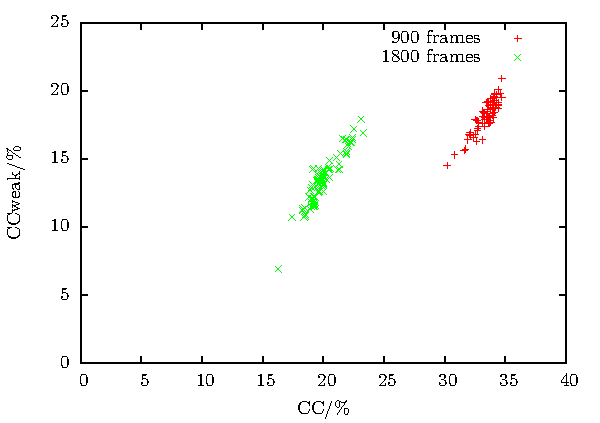
\includegraphics[scale=1.0]{figures/gold/cc_ccweak.pdf}
\end{center}
}

\frame{
\frametitle{Discussion}
\begin{itemize}
\item{Subset of data currently being used with native for structure
    solution}
\item{``Good'' solutions from SHELXD were verified to be correct}
\item{For reference: used zero-dose extrapolation in XSCALE, get 27.23
    / 13.57 for CC / CCweak}
\end{itemize}
}

\frame{
\frametitle{Conclusions}
\begin{itemize}
\item{This tool possibly most useful with shutterless data collection}
\item{Anisotropic diffraction: typically related to symmetry, symmetry
    used in calculation so not sure what effects are likely to be...}
\item{Makes no changes to the intensity values - only asks the
    question ``what happens if I stopped collecting earlier?''}
\item{Does not depend on an average value, only on differences between
    individual masurements}
\item{Makes no model of the radiation damage}
\item{Works with your existing software in a graceful way}
\end{itemize}
}

\frame{
\frametitle{Next step}
\begin{itemize}
\item{Extending to multi-crystal data analysis - all samples start at
    dose 0, may decay at different rates, total completeness
    available}
\end{itemize}
}

\frame{
\frametitle{Acknowledgements}
\begin{itemize}
\item{Support and input from Diamond Light Source and Diamond Staff}
\item{Miroslav Papiz, Steve Prince for converstion which got this
    started, inspriation for the name \emph{chef}}
\item{Kay Diederichs for $R_d$, as well as 0-dose with Sean McSweeney
    and Raimond Ravelli}
\item{Dave Stuart, Phil Evans for useful discussions on this subject}
\item{Ed Mitchell, I03 Staff, JCSG and Christian Siebold for the
    examples shown}
\end{itemize}
}

\frame{
\frametitle{Thank you}
}

\end{document}
